\documentclass[10pt,a4paper]{article}

\usepackage[utf8]{inputenc}
\usepackage[dutch]{babel}
\usepackage{fancyhdr}
\usepackage{geometry}
\usepackage{graphicx}
\usepackage{tabularx}
\usepackage{wallpaper}
\usepackage{listings}
\usepackage{amsmath}

\usepackage{xcolor, colortbl}
\definecolor{ugentblue}{HTML}{164A7C}
\definecolor{gray}{HTML}{AAAAAA}
\definecolor{lightgray}{HTML}{FAFAFA}
\definecolor{grayborder}{HTML}{CCCCCC}
\definecolor{commentgreen}{HTML}{009900}

% Tables
\def\arraystretch{1.35}
\renewcommand{\tabularxcolumn}[1]{>{\small}m{#1}}
\newcommand{\hcell}[1]{
	\cellcolor{ugentblue}\color{white}\textbf{#1}
}

\makeatletter
\renewcommand\thesubsection{\@arabic\c@section.\@arabic\c@subsection}
\makeatother{}

\usepackage[hypertexnames=false]{hyperref}
\usepackage[numbered, depth=3]{bookmark}

\renewcommand{\headrulewidth}{0pt}
\pagestyle{fancy}
\fancyhf{}

\interfootnotelinepenalty=0

% Listings
\lstset{
	backgroundcolor=\color{lightgray},
	basicstyle=\footnotesize,
	commentstyle=\color{commentgreen},
	frame=single,
	framesep=7pt,
	keywordstyle=\color{blue},
	language=Java,
	numbers=none,
	numbersep=5pt,
	numberstyle=\tiny\color{gray},
	rulecolor=\color{gray},
	stepnumber=1,
	stringstyle=\color{ugentblue},
	showspaces=false,
	showstringspaces=false
}

\begin{document}
	\begin{titlepage}
		%% Footer
		\thispagestyle{fancy}
		\fancyhf{}

		%% Page
		\hfill
		\begin{minipage}[t][0.9\textheight]{0.8\textwidth}
			\noindent
			
\includegraphics[width=55px]{ugent-blue.png} \\[-1em]
			\color{ugentblue}
			\makebox[0pt][l]{\rule{1.3\textwidth}{1pt}}
			\par
			\noindent
			\textbf{\textsf{Vage Databanken}} \textcolor{gray}{\textsf{Academiejaar 2014-2015}}
			\vfill
				\noindent
			{\huge \textsf{Project Vage Databanken}}
			\vskip\baselineskip
			\noindent
			\textsf{\textbf{Jasper D'haene} \\
				\textbf{Florian Dejonckheere}}
		\end{minipage}
	\end{titlepage}

	%%% PAGE STYLE %%%
	\nopagecolor
	\renewcommand{\footrulewidth}{0.4pt}
	\headheight 45pt
	\ULCornerWallPaper{1}{header.png}
	\fancyfoot[C]{\thepage}

	%%% DOCUMENT %%%
	\section{Generiek vaagregelsysteem}
		\noindent Beschrijving van het \texttt{FuzzySystem}. \\

		\noindent In het project werd gebruik gemaakt van een enkele extra library: de \href{https://commons.apache.org/proper/commons-math/}{Apache Commons Mathematics} library. Deze voorziet een stabiele numerieke implementatie van verscheidene integratiemethoden. Omdat de integratietijd belangrijker is dan de precisie, werd gekozen voor de simpelste implementatie: de \texttt{MidPointIntegrator}.

	\section{Controllers}
		\subsection{SafeController}
			\noindent Beschrijving van de \texttt{SafeController}.

		\subsection{SpeedController}
			\noindent Beschrijving van de \texttt{SpeedController}.

		\subsection{RallyController}
			\noindent Beschrijving van de \texttt{RallyController}.

	\section{Performantie}
		\subsection{Keuze t-norm en t-conorm}
			%% Is de keuze van t-norm en t-conorm belangrijk voor de prestatie (i.e. de gemiddelde snelheid) van de wagen?

		\subsection{Robuustheid regelsysteem}
			%% Hoe robuust is uw regelsysteem voor verschillende races? Is de gemiddelde snelheid ongeveer dezelfde als u de wagen verschillende keren laat racen op een welbepaald parcours?

		\subsection{Minder performante parcours}
			%% Zijn er parcours waar uw controller minder goed presteert? Hoe komt dit?
			\noindent Bepaalde parcours zijn zo geschreven dat de sensoren af en toe tekort komen. In een scherpe bocht bijvoorbeeld, kan het zijn dat de vooruitkijkende sensoren de bocht niet opmerken (voornamelijk door de hogere snelheid), en een foutieve meting geven voor de wand ertegenover.

			\begin{figure}[h]
				\centering
				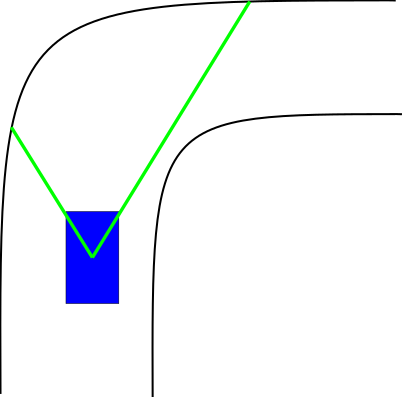
\includegraphics[width=5cm]{sensors-corner.png}
				\caption{Foutieve meting bij scherpe bochten}
				\label{fig:sensors-corner}
			\end{figure}

			\noindent Op zich kan dit probleem verholpen worden door de hoek van de sensoren continu adaptief aan te passen -- zodat een scherpe bocht toch opgemerkt wordt -- ware het niet dat de outputvariabelen van een bepaalde iteratie geen enkele invloed hebben op de volgende iteratie. Opnieuw kan dit probleem suboptimaal opgelost worden door het intelligent gebruik maken van \textit{dampening}, waarbij beslist wordt of de output van de huidige iteratie authoritatief wordt doorgevoerd, of dat de vorige iteratie er invloed op hebben. Een goede optimalisatie voor dit karakter is een lokale \textit{cache} van sensoren, zodat het patroon van een semi-zichtbaar obstakel kan gedetecteerd worden. Dit systeem valt echter niet in de scope van dit project en werd dus ook enkel als gedachte-experiment aangehaald.

			\noindent Uiteindelijk werd gekozen om een vaste sensorhoek te hanteren, bepaald uit empirische experimenten op verschillende parcours met verschillende controllers.

		\subsection{Veiligheid}
			%% Hoe veilig is uw wagen, i.e. hoe dikwijls crasht uw wagen?

		\subsection{Exacte controller}
			%% Wat zijn de verschillen met een exacte controller (beter/slechter)?
			\noindent Een exacte controller reageert volgens welbepaalde scherpe grenzen op de input. Het grote verschil met deze systemen is dat er van een graduele aanpak geen sprake kan zijn. Bij een vaag regelsysteem kan de granulariteit van de response aangepast worden volgens constanten of andere (input-) parameters. Er kunnen meerdere regels zijn die betrekking hebben op \'e\'en aspect, en die dus elk tot op een bepaalde mate invloed hebben op de uitkomst van het systeem. \\

			\noindent Beschouw het volgende systeem met als output \texttt{acceleration}: Als er zich geen obstakels bevinden voor de auto, kan hij versnellen. Maar de versnelling moet gematigd zijn als de auto aan het driften is (dus als de laterale snelheid groter dan 0 is).
			Dit kan eenvoudig gemodelleerd worden door de volgende regels.

			\begin{lstlisting}
IF (distanceFront IS SMALL) THEN acceleration IS high
IF (lateralVelocity IS GREATER THAN ZERO) THEN acceleration IS low
			\end{lstlisting}

			\noindent Door het combineren van deze regels wordt in een drift rekening gehouden met zowel \texttt{acceleration IS high} en \texttt{acceleration IS low}, waardoor een gebalanceerd equilibrium uiteindelijk gekozen wordt als \texttt{acceleration}.
			Indien men dit in een exacte controller wil implementeren, moeten de twee regels gemultiplexd worden in \'e\'en formule. Dit kan bijvoorbeeld als volgt gebeuren.

			\begin{lstlisting}
int factor = 1;
if (lateralVelocity > 0)
	factor = 0.5;

return (1400 * (distanceFront / 200) * factor);
			\end{lstlisting}

			\noindent Deze formule bevat significant meer complexiteit en is ook sensitiever dan een vaagregelsysteem. Ook als er (foutieve) waarden optreden die buiten het definitiegebied vallen, kan de output een ongewenste waarde aannemen. Vage regelsystemen hebben hiertegen een intrinsieke bescherming, aangezien $\mu = 0$ buiten het definitiegebied van de lidmaatschapsfunctie.
\end{document}
